\documentclass[11pt, a4paper, norsk]{NTNUoving}
\usepackage[utf8]{inputenc}
\usepackage[T1]{fontenc}
\usepackage{mathrsfs}
\newcommand{\RomanNumeralCaps}[1]
{\MakeUppercase{\romannumeral #1}}


\ovingnr{6}    % Nummer på innlevering
\semester{Haust 2022}
\fag{TMA4120}
\institutt{Institutt for matematiske fag}

\begin{document}
\section*{12.6}
\begin{oppgave}[11]
  Vi har oppgitt en del informasjon:
  \begin{align*}
    u_x(0,t) &= u_x(L, t) = 0 \\
    u(x, t) &= f(x) \\
    u_t &= c^2 u_{xx}
  \end{align*}
  Lar $u(x,t) = F(x)G(t)$, som gir
  \begin{align*}
    F''+p^2F &= 0 \\
    G' c^2 p^2 G &= 0
  \end{align*}
  Kan løse for $F$
  \begin{align*}
    F(x) &= A\cos(px)+B\sin(px) \\
    F'(x) &= -pA\sin(px)+pB\cos(px)
  \end{align*} 
  Setter inn initialbetingelser, som gir
  \begin{align*}
    F'(0) &= pB = 0 && \Rightarrow B = 0 \\
    F'(L) &= -pA\sin(pL) && \Rightarrow p = \frac{n\pi}{L}
  \end{align*} 
  Løser tilsvarende for $G$, og står igjen med 
  \[
    u_n(x,t) = F_n(x)G_n(t)=A_n\cos\frac{n\pi x}{L} e^{-\lambda_n^2t}
  \]
  der $\lambda_n = \frac{c n \pi}{L}$, slik at
  \[
    u(x,t) = \sum_{n=0}^\infty u_n(x,t)
    = \sum_{n=0}^\infty \cos\frac{n\pi x}{L} e^{-(cn\pi/L)^2t}
  \]  
  Gitt at $u(x,t)=f(x)$, ser vi at $A_n$ tilsvarer Fourierkoeffisientene til $f(x)$, og kan uttrykkes som oppgave ber om. 
\end{oppgave}
\newpage
\begin{oppgave}[12]
  Vi har gitt $f(x)=x$, og kan løse oppgaven ved å finne Fourierkoeffisientene.
  \begin{align*}
    A_0 &= \frac{1}{\pi} \int_0^\pi x dx = \frac{\pi}{2} \\
    A_n &= \frac{2}{\pi} \int_0^\pi x \cos(nx) dx = \frac{2\cos(\pi n)-2}{\pi n^2}
  \end{align*}
  Skriver ut noen ledd av summen
  \[
    u(x,t) = \frac{\pi}{2} - \frac{4}{\pi} \left[
   \cos(\pi x)e^{-t}+\frac{1}{9}\cos(3\pi x)e^{-9t}+\frac{1}{25}\cos(5\pi x)e^{-25t}+...
  \right]
  \]  
  Plotter funksjonen i python for å se tidsutviklingen
  \[
    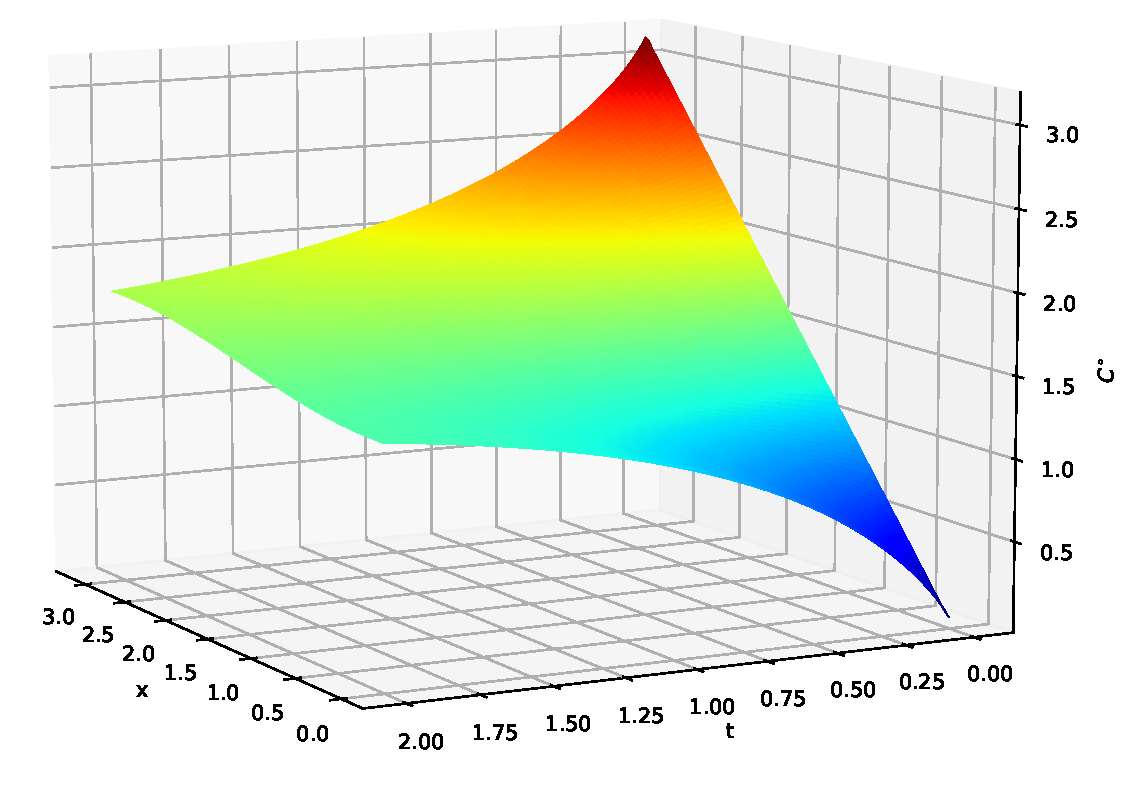
\includegraphics[scale=0.4]{12.6.12__3D.pdf}
  \]
\end{oppgave}
\begin{oppgave}[14]
  Vi har gitt $f(x)=\cos(2x)$, og kan løse oppgaven ved å finne Fourierkoeffisientene.
  \begin{align*}
    A_0 &= \frac{1}{\pi} \int_0^\pi \cos(2x) dx = 0 \\
    A_n &= \frac{2}{\pi} \int_0^\pi \cos(2x) \cos(nx) dx = 1 , n=0 
  \end{align*}
  Vi kjenner til siste integralet, som er null i alle verdier utenom $n=2$, da det blir 1. Dette gir den noe enkle funksjonen
  \[
    u(x,t) = \cos(2\pi x)e^{-2t} 
  \]  
  Plotter funksjonen i python for å se tidsutviklingen
  \[
    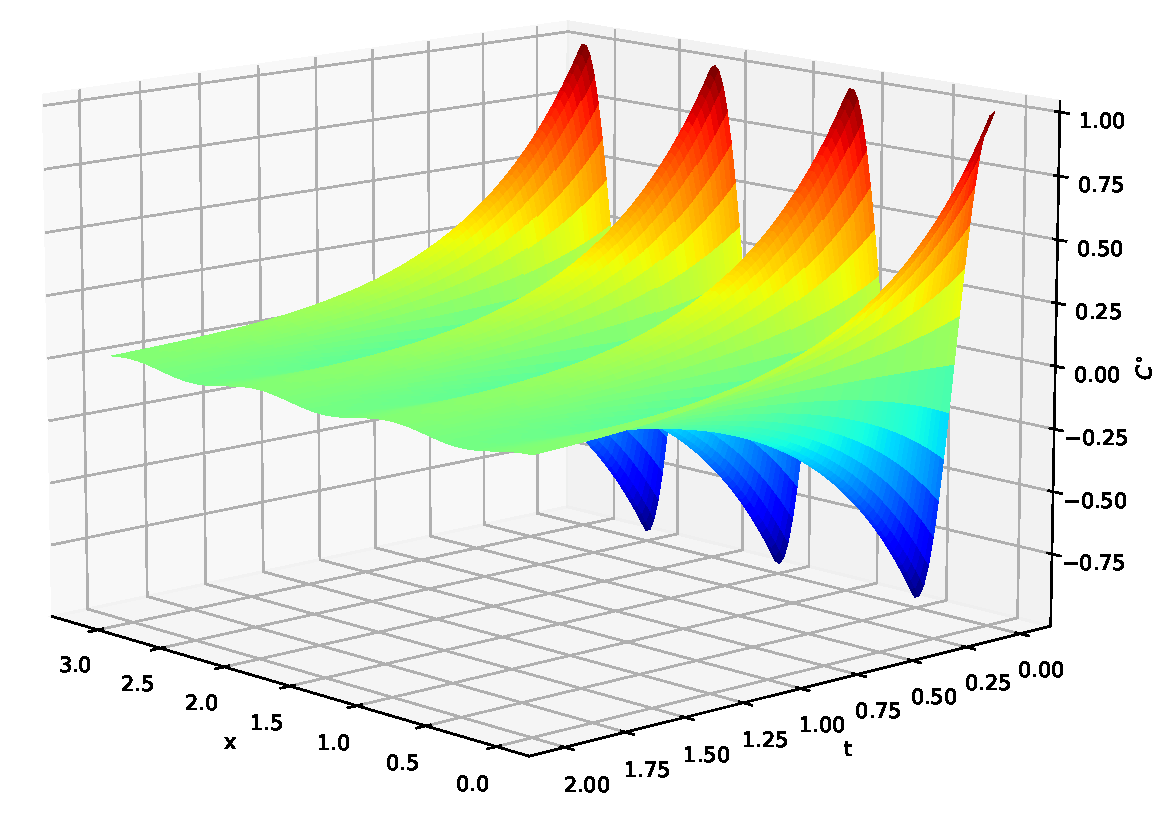
\includegraphics[scale=0.4]{12.6.14__3D.pdf}
  \]
\end{oppgave}
\newpage
\begin{oppgave}[16]
  Nytter hintet, som sier at $u = v - Hx(x-\pi)/(2c^2)$. Setter dette inn i den oppgitte differensialligningen $u_t = u_{xx} + H$.
  \begin{align*}
    u_t &= v_t \\
    u_{xx} &= v_{xx} - \frac{H}{c^2} \\
    \Rightarrow v_t &= c^2\left(v_{xx}-\frac{H}{c^2}\right)+H = c^2 v_{xx}
  \end{align*}
  Ser at vi får varmeligningen på en form vi kjenner til. Løsningen blir som vanlig
  \[
    v(x,t)=\sum_{n=0}^\infty B_n\sin\frac{n\pi x}{L} e^{-\lambda^2t}
  \]
  med $B_n=\frac{2}{\pi}\int_0^\pi g(x)\sin(nx) dx$. Gitt $u(x,0) = f(x)$ definerer vi 
  \[
    f(x) = v(x,0) - Hx(x-\pi)/(2c^2) \Rightarrow g(x) = u(x,0) + Hx(x-\pi)/(2c^2)
  \]
\end{oppgave}
\begin{oppgave}[21]
  Bruker varmeligningen for to dimensjoner:
  \begin{align*}
    \frac{\partial u}{\partial t} = c^2 \nabla^2 u
    && \nabla^2u=\frac{\partial^2u}{\partial x^2} + \frac{\partial^2u}{\partial y^2}=0
  \end{align*}  
  Antar $u(x,y) = F(x)G(y)$, som ved Laplaceligningen gir
  \begin{align*}
   \frac{1}{F}\frac{d^2F}{dx^2} = -\frac{1}{G}\frac{d^2G}{dy^2} = -k 
  \end{align*}
  Ved initialbetingelsene blir dette
  \begin{align*}
    F_n(x) &= B\sin\frac{n\pi x}{a} \\
    G_n(y) &= A_ne^{n\pi y/a}-A_ne^{-n\pi y/a} = 2A_n \sinh\frac{n\pi y}{a}
  \end{align*}
  Videre har vi
  \[
    u(x, a) = f(x) = \sum_{n=1}^\infty C_n \sin\frac{n\pi x}{a} \sinh(n\pi) 
  \]
  $C_n$ i lag med $\sinh$ faktoren, utgjør Fourierkoeffisientene til $f(x)$, som kan løses ved
  \[
    C_n = \frac{2}{\sinh(n\pi)}\int_0^a f(x)\sin\frac{n\pi x}{a} dx
  \] 
  Med $a=24$ og $f(x)=25$, blir den ferdige løsningen
  \[
    u(x,t)=\frac{100}{\pi}\sum_{n=1, n \text{  odde}}^\infty \frac{1}{n\sinh(n\pi)}\sin\frac{n\pi x}{24}\sinh\frac{n\pi y}{24}
  \]  
  Lager et heatmap i python for å illustere/verifisere løsningen
  \[
    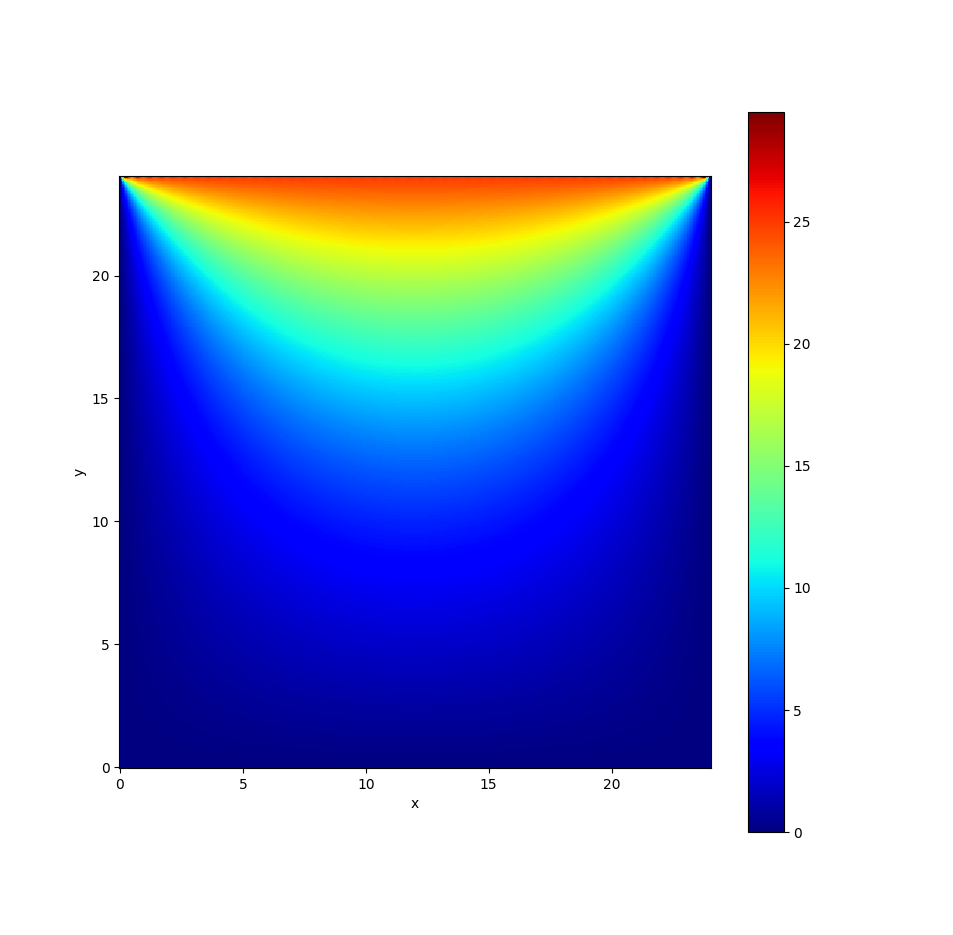
\includegraphics[scale=0.5]{Figure_1.png}
  \]  
\end{oppgave}
\section*{12.7}
\begin{oppgave}[1]
  Bruker Fouriertransformasjon på ligningen:
  \begin{align*}
    2u_x+3u_t = 0 &\Rightarrow 3\mathcal{F}(u_x)+2\mathcal{F}(u_t) = 0 \\
    &\Rightarrow \mathcal{F}(u_t) = -\frac{2}{3} w i \hat{u}
  \end{align*}
  Kan vise at Fouriertransformasjonen ser over derivasjon med hensyn på tid, og får
  \[
    \frac{\partial\hat{u}}{\partial t} = -\frac{2}{3} w i \hat{u}
  \]  
  Løser denne, som gir
  \[
    u(x,t) = C(w)e^{-\frac{2}{3}iwt}
  \]
  Med $u(x,0) = f(x)$ ser vi at $C(w) =\hat{f}(w)$.
  \begin{align*}
    u(x,t)&=\frac{1}{\sqrt{2\pi}}\int_{-\infty}^\infty\hat{f}(x)e^{-\frac{2}{3}iwt}e^{iwx}dw \\
          &=\frac{1}{2\pi}\int_{-\infty}^\infty f(v) \int_{-\infty}^{\infty}e^{-\frac{2}{3}iwt}e^{i(wx+wv)}dw dv \\
     &=\frac{1}{2\pi}\int_{-\infty}^\infty f(v) \int_{-\infty}^{\infty}e^{-\frac{2}{3}iwt}[\cos(wx+wv)+i\sin(wx+wv)]dw dv \\
     &=\frac{1}{\pi}\int_{-\infty}^\infty f(v) \int_{0}^{\infty}e^{-\frac{2}{3}iwt}\cos(wx+wv)dw dv 
  \end{align*}
  Dette kan løses for en gitt $f(x)$, som igjen vil løse differensialligningen for $u(x,t)$.
\end{oppgave}
\begin{oppgave}[2]
  Går frem helt tilsvarende forrige oppgave. Til å begynne med finner vi Fouriertransformen til ligningen, og løser denne. Transformasjon gir
  \[
    \frac{\partial\hat{u}}{\partial t} = -\frac{2}{3}iwt\hat{u}
    \Rightarrow \hat{u} = \hat{f}(w)e^{-\frac{1}{3}iwt^2}
  \]  
  Bruker samme argumentasjon som i forrige oppgave
  \[
    u(x,t) = \frac{1}{\pi}\int_{-\infty}^\infty f(v)\int_0^\infty e^{-\frac{1}{3}iwt^2}\cos(wx+wv)dw dv
  \]
\end{oppgave}
\begin{oppgave}[3]
  Med samme metode som i de forrige oppgavene, har vi
  \[
    u(x,t)=\frac{1}{\sqrt{2\pi}}\int_{-\infty}^\infty\hat{f}(w)e^{-\frac{1}{2}w^2t^2}e^{iwx}dw
  \]
  Definerer
  \[
    \hat{g}(w)=e^{-\frac{1}{2}w^2t^2}
  \]  
  slik at
  \[
    u(x,t)=(f*g)(x)=\int_{-\infty}^\infty \hat{f}(w)\hat{g}(w)e^{iwx}dw
  \]  
  Ved definisjon av konvolusjon har vi
  \[
    (f*g)(w)=\int_{-\infty}^\infty f(x-s)g(s) ds
  \]
  Litt usikker på hvorfor det står $f(x-st)$ i oppgaveteksten, og jeg klarte ikke vise dette, men tar utgangspunkt i konvolusjonen over likevel. Kan med dette avgjøre $g(s)$. Bruker formelen
  \[
    \mathcal{F}\left(e^{-ax^2}\right)=\frac{1}{\sqrt{2a}}e^{-w^2/(4a)}
  \]
  Dette passe oss godt dersom $a=1/(2t^2)$, slik at
  \[
    \mathcal{F}\left(e^{-x^2/(2t^2)}\right)=te^{-\frac{1}{2}w^2t^2)}=t\hat{g}(w)
  \]
  Dermed har vi funnet inversen til $\hat{g}(w)$, som er
  \[
    g(x) = \frac{1}{t}e^{-(x/t)^2/2} 
  \]
  som gir
  \[
    u(x,t)=\frac{1}{\sqrt{2\pi}t}\int_{-\infty}^\infty f(x-s)e^{-(x/t)^2/2}
  \]
\end{oppgave}  
\end{document}